\documentclass[12 pt]{article}
\usepackage{hyperref, fancyhdr, setspace, enumerate, amsmath,
  lastpage, amssymb}
\usepackage[margin=1 in]{geometry}
\allowdisplaybreaks
%\usepackage[dvipsnames]{xcolor}   %May be necessary if you want to color links
\hypersetup{
	%colorlinks=true, %set true if you want colored links
	linktoc=all,     %set to all if you want both sections and subsections linked
	linkcolor=black,  %choose some color if you want links to stand out
}
\usepackage{graphicx}
\graphicspath{{Images/}}
% Independent symbol
\newcommand\independent{\protect\mathpalette{\protect\independenT}{\perp}}
\def\independenT#1#2{\mathrel{\rlap{$#1#2$}\mkern2mu{#1#2}}}
\author{Julian Lore}
\date{Last updated: \today}
\title{MATH 324: Statistics}
\pagestyle{fancy}
\lhead{MATH 324}
\chead{\leftmark}
\rhead{Julian Lore}
\cfoot{Page \thepage \ of \pageref{LastPage}}
\newcommand{\tab}[1]{\hspace{.2\textwidth}\rlap{#1}}
\begin{document}
	\onehalfspacing
	\maketitle
	Notes from Masoud Asgharian's Winter 2018 lectures.
	\tableofcontents
        \section{01/09/18}
        \paragraph{What we will cover this semester}
        Will essentially cover chapter 8,9,10. For chapter 11, he will
        give us his own notes. The first 6 sections of chapter 13 and
        a few sections from chapter 14. Occasionally we will go back
        to chapter 7 to revisit things like the t distribution.
        \\ In 323, we made probabilistic models. Statistics is the
        breach in which we connect these models to real
        life. Otherwise, those are just models. A core part of data
        analysis and data sciences is statistics and computer
        science.
        \subsection{Overview - What is Statistics?}
        Inductive logic, we have a sample from the population we want
        to make inference about. With this data, we want to extend the
        results to the whole population. From small to large, sample
        to the population.
        % Image
        \\ 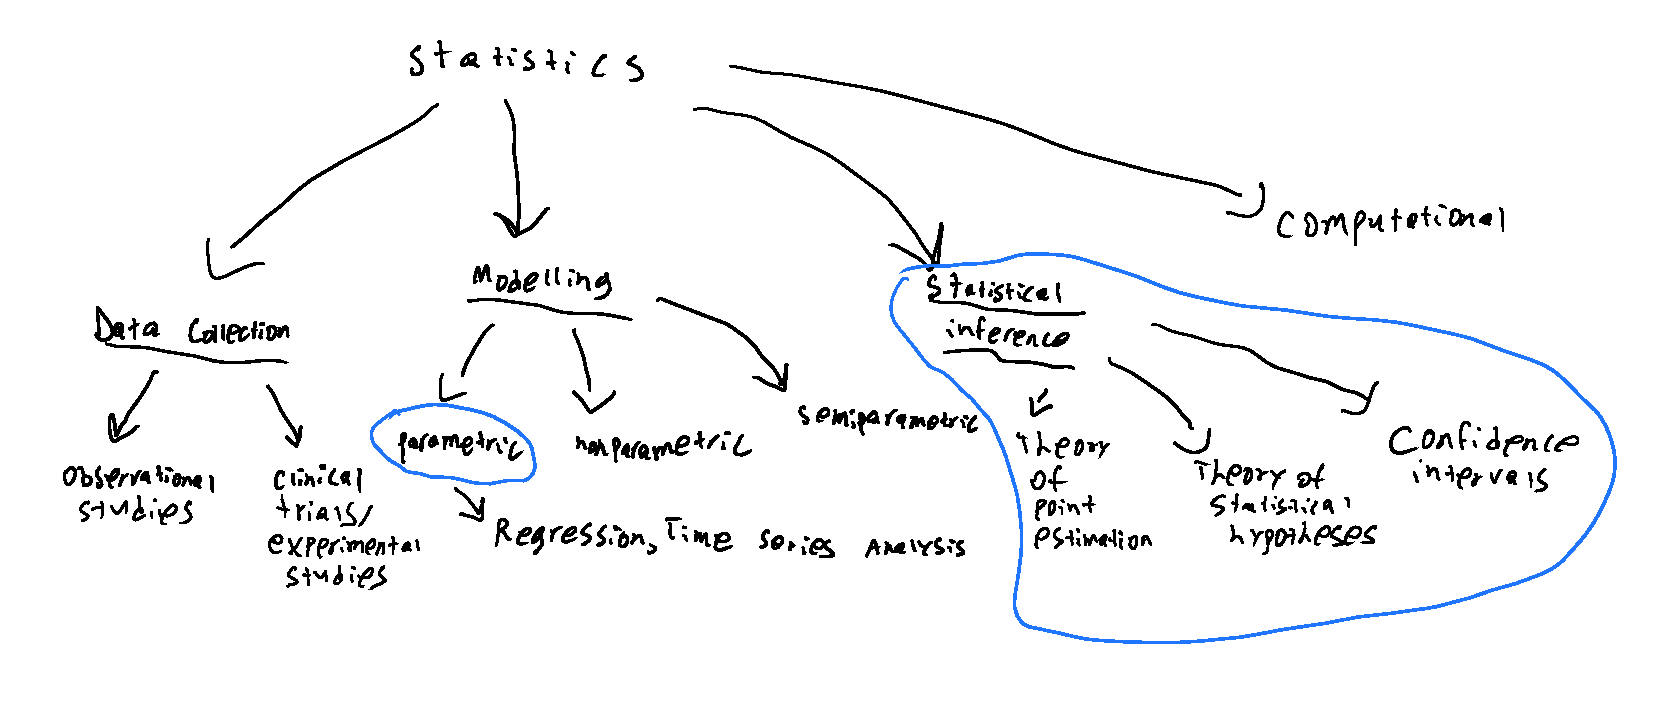
\includegraphics[width=\textwidth]{i1.pdf}
        \begin{itemize}
        \item Observational studies: we go to the population and make
          observations.
        \item Experimental studies: give test subjects something,
          i.e. give them cigarettes when trying to test for if
          cigarettes lead to cancer. Need
          to account for causation, other factors that can affect
          outcome. In order to do so we have to keep their diet and
          other factors controlled. We must also have some sort of
          randomization, we can't send all males to one group and all
          females to another, as males may have a tendency to smoke or
          something of the like. These are also called clinical
          trials.
        \item When we have data, the next step is modeling. May
          occasionally speak of this, but this is not part of the
          course. There are different approaches to modeling, can be
          split into 3 parts.
          \begin{itemize}
          \item Parametric: the salary is distributed like a
            distribution (ex. Gamma), but we don't know the
            parameters. Take for example, we always know that the
            normal distribution is a bell curve, but we don't know
            where it's centered. Very useful, but we might have a
            miss-specification. How do we know our models are correct?
            Most of the time we will be talking about
            \textbf{parametric} models.
          \item Semiparametric
          \item Nonparametric: since we don't know if parametric
            models are correct, we make no assumption about the
            distribution. We just assume that $X \sim F$, all we
            assume about $F$ is that it's continuous, nothing
            more. This is an infinite dimensional vector. Why? How do
            we know a function? We have a vector for $F$, like
            $F(1),F(2, \ldots)$. How do we approximate this? $X_i
            \stackrel{iid}{\sim}F, i=1,2,\ldots,n$. $n$ patients, with
            all the same distribution. So $F(t)=P(X\leq t)$. What does
            this tell us? The proportion of time that $x$ falls below
            $t$. So with $n$ samples, how do we mimic this? We count
            the number of observations below $t$, i.e. $\frac{\#X_i
              \leq t}{n}$, which is an approximation of the
            above. This is an empirical observation. More
            mathematically:
            \begin{equation*}
              \varepsilon(t) =
              \begin{cases}
                1 & \text{if }t\geq 0
                \\ 0 & \text{otherwise}
              \end{cases}
            \end{equation*}
          So we have
          $\hat{F}_n(t)=\frac{1}{n}\sum_{i=1}^n\varepsilon(t-x_i)$. This
          gives us a binomial distribution. But we are assuming they
          are all the same distribution.
          \\ Nonparametric approaches are good for functions of single
          variables, but not for multi variables, which is what
          semiparametric was made for.
          \end{itemize}
          \item Bayesian inference: when you learn that $X \sim N(\mu,
            \sigma^2)$, $X$ is normally distributed and $\mu$ is the
            average of the whole population. Bayes' approach says that
            these parameters are not constants, these are random
            variables themselves. Bayes did not look at probability as
            a frequentest approach, not the proportion of when something
            arrives (frequentest approach works when we have a huge
            sample). The other approach that Bayes had was an updating
            approach, that our parameters are unknown. This is good
            for when you have a stream of data (machine learning is a
            prime example). We have a lack of knowledge and then we
            update it using Bayesian's approach. $\to X | \mu,
            \sigma^2 \sim N (\mu, \sigma^2)$, i.e. the parameters are
            also normally distributed.
          \end{itemize}
          Most of the time we'll be at parametric modeling and
          statistical inference.
        \subsection{Point Estimation} What do we mean by point
        estimation? A scientific guess about the unknown parameter of
        the population. Consider the following situation:
        \\ $x_1, \ldots, x_n \sim N(\mu, 1)$ (usually interested in
        the normal distribution, binomial and poisson). Suppose this
        is the IQ of high school graduates in Canada (the $X_i$ are
        numbers). Why do we call this distribution normal? Because for
        a healthy population, most of the weight should be in the
        middle, just like the bell curve. The Normal distribution is
        especially important for modeling error. For insurance
        companies, we see at the tails that there aren't many large
        claims.
        \\ We want to find $\mu$. Recall that $E(X_i)=\mu,
        i=1,2,\ldots,n$ (if they all have the same observations, they
        have the same mean).
        \\ First, what is a point estimation? What properties should
        it have? If we know the value of $\mu$, we have the whole
        thing, can calculate everything. How do we estimate this? The
        whole population is huge, so we take a sample part of the
        population, mimicking the real $\mu$, getting $\overline{X}_n
        = \frac{1}{n}\sum_{i=1}^nX_i$. $\overline{X}_n$ is useful, but
        $\overline{X}_n-\mu$ isn't, as there's an unknown we have
        here.
        \paragraph{Statistic} A function of observations that does not
        depend on any unknown parameter.
        \subparagraph{Ex} $\overline{X}_n$ is a
        statistic. $\overline{X}_n - \mu$ is not.
        \paragraph{Estimator} A statistic that aims at estimating an
        unknown parameter (we want to work with it). For example, if
        $\mu$ moves from $-\infty$ to $\infty$, we want to have an
        estimator that also has the same range, not one that is
        strictly positive. Example: $\overline{X}_n$ is an
        estimator. However, consider:
        $$S^2 = \frac{1}{n-1}\sum_{i=1}^n(X_i-\overline{X}_n)^2$$
        This is a statistic, but not an estimator, it always returns a
        positive value. Also, take for example in physics, where each
        measure has a unit of measurement. This statistic wouldn't
        even be the same unit, so it once again is a bad estimator.
        \\ When we take a mean and try to estimate it, the next step
        is to figure out how we quantify possible bias.
        \\ \rule{\textwidth}{0.5 pt}
        $$\varepsilon = |\overline{X}_n-\mu |$$
        We can use Tchbycshev's inequality to put a bound on the
        error.
        \begin{flalign*}
        P(|X-\underbrace{E(X)}_{\mu_x}|>k\sqrt{\underbrace{Var(X)}_{\sigma_x^2}})
        \\ P(|X-\mu_x>k\sigma_x) \leq \frac{1}{k^2}
        \end{flalign*}
        Very useful, assume very little but get lots of
        information. One of the big hammers of probability and
        statistics. The only thing we assume here is the existence of
        the second moment.\\
        Consider $k=3$.
        \begin{flalign*}
          P(|X-\mu_x|>3\sigma_x)\leq \frac{1}{9}
          \\ P(|X-\mu_x|\leq 3 \sigma_x)\geq 1 - \frac{1}{9}\approx \%89
        \end{flalign*}
        Without knowing anything else about the distribution, this
        tells us that about $89\%$ of the population is within $3$
        times the variance of the mean.
        \section{01/11/18}
        Last lecture we learned about statistics, estimators and how
        we can measure deviation from the target and the estimation.
        \\ We had $n$ random variables: $x_1, \ldots, x_n, \mu
        \rightarrow$ IQ in the population. We want to have a
        scientific guess of the average IQ (there are many more
        examples, like salary). Our $n$ random variables are $n$
        random people chosen.
        \\ We then arrive at $\overline{X}_n =
        \frac{1}{n}\sum_{i=1}^nX_i$, a scientific guess mimicking
        $\mu$ but in the sample population.
        \\ How much deviation do we have? $|\overline{X}_n - \mu|$
        \\ Since our observations are random, then $\overline{X}_n$
        will also be random, i.e. $\overline{X}_n$ is a random
        variable itself. Each person gives us a different deviation,
        so we need a way to summarize all of this information, say,
        the expected value.
        $$ E[|\overline{X}_n - \mu |]$$
        Another way to summarize it is with probability.
        $$ P(|\overline{X}_n - \mu | > \varepsilon)$$
        What is the chance that what we produce is not within
        $\varepsilon$ of the target? Often times we want to bound
        these things. What do you think might happen if instead of
        taking a sample of $n=50$, we take $n=100$? As $n$ increases,
        we should get closer to the target. But, the more samples I
        take, the more it'll cost me. So we want to have a balance. We
        want the distance from the target to be within some sort of
        value.
        $$P(| \overline{X}_n - \mu| > \varepsilon) \leq \delta$$
        Take for example a spam filter. Something is either spam or
        not spam. We start with messages and then start checking. We
        want to know how many messages we should check, i.e. how big
        our training set should be.
        \\ We will use Tchbycshev's Inequality for this!
        \subsection{Chebyshev/Tchbycshev's Inequality}
        Let $X$ be a random variable. Suppose $h(x)$ is a positive
        function (i.e. the range of this function consists of positive
        values). We can show that
        $$P(h(x) \geq \lambda) \leq \frac{E[h(x)]}{\lambda}$$ for any
        $\lambda >0$, if $E[h(X)] \leq \infty$, i.e. it exists. This
        is called \textbf{Markov's Inequality}
        \\ When we say that the expected value of a random variable
        exists, we mean $E[|X|] < \infty$. When we talk about
        existence of a moment, we check the absolute value, but the
        actual value does not have an absolute value, it is just
        $E[X]$. Why? The trouble is when $X$ can take positive and
        negative values and is not bound.
        \begin{flalign*}
          E[X] & = \sum_{i=1}^\infty X_i P(X=x_i) &
        \end{flalign*}
        What if we have infinite values that we can take?
        \paragraph{Recall from Calculus}
        $\sum_{n=1}^{\infty} \frac{(-1)^n}{n}<\infty$ is convergent,
        but not absolutely convergent because $\sum_{n=1}^\infty
        \left| \frac{(-1)^n}{n}\right| = \infty$. Riemann has a result
        such that if a series is convergent but not absolutely
        convergent (like the example just mentioned), then it can
        converge to any real number (if we reorder the terms). Thus we
        don't like this and must check for absolute convergence for
        moments, or else the expected value will depend on the order
        we consider the numbers in.
        \\ Recall the theorem that says if we have a function of a
        random variable, we don't need its distribution, we can
        directly use the distribution of $X$. Note that integrals are
        another form of sums, we can use similar notation with $x$ as
        a subscript to denote ranging over all $x$.
        \begin{flalign*}
          E[h(x)] & = \int_{x} h(x)f_x(x) \ dx = \left(\int_{x : h(x) \geq \lambda} + \int_{x:h(x) < \lambda}h(x)f_x(x) \ dx\right) &
          \intertext{(Note that the two integrals both apply on the
            right side)}
          & \geq \int_{x:h(x) \geq \lambda}h(x)f_x(x)\ dx \geq \lambda \int_{x: h(x) \geq \lambda} f_x(x)\ dx = \lambda P(h(x) \geq \lambda)
        \end{flalign*}
        So what did we get?
        \begin{flalign*}
          E[h(x)] & \geq \lambda P(h(x)\geq \lambda) &
          \\ P(h(x) \geq \lambda) & \leq \frac{E[h(x)]}{\lambda}
        \end{flalign*}
        Now consider: $h(x) = (x-\mu)^2$. Then what do we have?
        \begin{flalign*}
          P(|x-\mu| \geq \lambda) &= P([x-\mu]^2 \geq \lambda)
          \stackrel{\text{By Markov's Inequality}}{\leq}\frac{E[(x-\mu)^2]}{\lambda^2} &
          \\ P(|x-\mu| \geq \lambda)&\leq \frac{Var(x)}{\lambda^2}
          \intertext{Replace $\lambda$ by $k\sigma_x$ where $\sigma_x=\sqrt{Var(x)}$}
          \intertext{$k$ is a constant, so we get:}
          \\ P(|x-\mu| \geq k \sigma_x) &\leq \frac{Var(x)}{k^2\sigma_x^2}=\frac{Var(x)}{k^2 Var(x)} = \frac{1}{k^2}
        \end{flalign*}
        This is \textbf{Tchbycshev's Inequality}. For $k=3$ we have:
        \begin{flalign*}
          P(|x-\mu| \geq 3 \sigma_x) &\leq \frac{1}{9}
          \\ P(|x-\mu| \leq 3\sigma_x)&\geq \frac{8}{9} \approx 88\%
        \end{flalign*}
        What does this say? For any random variable with $2$ moments,
        88\% of the values fall within $3 \sigma_x$s from the center
        of gravity (mean). This is a very crude lower bound that
        required almost no assumptions, all we need is that $\mu =
        E(x)$ and $\sigma_x^2 = Var(x)$ and the existence of the
        second moment.
        \\ Back to where we were before with $|\overline{X}_n - \mu|$:
        \begin{flalign*}
          P(|\overline{X}_n - \mu| > 3\sigma_{\overline{X}_n}) \leq \frac{1}{9} &
        \end{flalign*}
        Note that here, it must be true that $\mu =
        E(\overline{X}_n)$. Is this true?
        \begin{flalign*}
          \overline{X}_n &= \frac{1}{n}\sum_{i=1}^n X_i &
          \\ E[\overline{X}_n] &= E\left[\frac{1}{n}\sum_{i=1}^n X_i\right]
          \intertext{Recall: $E[cY] = cE[Y]$, think of expected values
            like integrals and sums, they have the same properties.}
          \\ & = \frac{1}{n} E\left[\sum_{i=1}^n X_i\right] = \frac{1}{n}\sum_{i=1}^n E[X_i]
          \intertext{Remember that $X_1, \ldots, X_n \sim F$,
            i.e. they all have the same distribution! So $E[X_i]=\mu, i=1,2,\ldots,n$}
          \\ & = \frac{1}{n}\sum_{i=1}^n \mu = \mu
        \end{flalign*}
        Now how do we use this in practice? If everyone is sent to the
        population and asked to take a sample of size $10$ (the same
        size for everyone) and everyone makes their own
        $\overline{X}_n$, their own sample average and then we take
        the average of all the sample averages and we obtain the
        actual average of the population, i.e. this is an average of
        averages (this is difficult though, as we need all the
        possible averages of size $10$; in practice we only use one
        sample, more on this later).
        \paragraph{Example}
        Suppose we have the following $0$-$1$ random variable
        representing what people will vote for
        \begin{equation}
          X_i =
          \begin{cases}
            1 & \text{if NDP}
            \\ 0 & \text{otherwise}
          \end{cases}
          \end{equation}
          We know that $X_i \sim$ Bernoulli($p$), $p=P(X_i=1)$
          \begin{flalign*}
            X_1,\ldots,X_n \sim p=(P(X_i=1),i=1,2,\ldots,n) &
          \end{flalign*}
          \begin{flalign*}
            \overline{X}_n = \frac{1}{n}\sum_{i=1}^n X_i = \hat{p}_n
          \end{flalign*}
          \paragraph{Side Note about Picking with Replacement}
          \begin{flalign*}
            P(X_2 = 1 | X_1 = 1) & = \frac{M-1}{N-1}
          \end{flalign*}
          (after taking $1$ in favor of NDP, where $N$ is total
          population size and $M$ is total number of people in favor
          of NDP) Using Total Probability Theorem we get:
          \begin{flalign*}
            P(X_2 = 1) & = P(X_2 = 1 | X_1 = 1)P(X_1 = 1) + P(X_2 = 1 | X_1 = 0)P(X_1 = 0)
            \\ & = \frac{M-1}{N-1}\cdot \frac{M}{N}+\frac{M}{N-1}\left(1 - \frac{M}{N}\right) = \frac{M}{N}
            \\ P(X_2 = 1)&=\frac{M}{N}
            \\ P(X_2 = 1 | X_1 = 1)&=\frac{M-1}{N-1}
          \end{flalign*}
          These are identically distributed, but not independent, this
          replacement is what differs hypergeometric from
          binomial. But when the sample size is very large we can just
          use binomial (also we don't ask someone who they're voting
          for twice).
          \\ \rule{\textwidth}{0.5pt}
          Note we just showed that
          \begin{flalign*}
            P(|\overline{X}_n - \mu | > k \sigma_{\overline{X}_n}) &\leq \frac{1}{k^2}&
            \intertext{Recall that if $X_i \sim$ Bernouilli($p$), then
              $E[X_i]=p$}
            P(|\overline{X}_n - \mu | \geq k \sigma_{\overline{X}_n}) & = P(|\hat{p}_n - p| > k\sigma_{\hat{p}_n})
          \end{flalign*}
          Recall that:
          \begin{flalign*}
            \sigma_{\overline{X}_n}^2 &= Var(\overline{X}_n) &
            \\ Var(c Y) & = c^2 Var(Y)
            \\ Var(X\pm Y) & = Var(X) + Var(Y) \pm 2 Cov(X,Y)
          \end{flalign*}
          If $Cov(X,Y)=0$, $Var(X \pm Y)=Var(X)+Var(Y)$. If $X$ and $Y$
          are independent, $Cov(X,Y)=0$.
          \begin{flalign*}
            Cov(X,Y) & = E(XY) - E(X)E(Y) &
            \\ X \independent Y \implies E[g(x)h(y)]&=E[g(x)]E[h(y)]
            \\ X \independent Y \implies E(XY) &= E(X)E(Y) \text{
              therefore }Cov(X,Y)=0
          \end{flalign*}
          Thus,
          \begin{flalign*}
            Var(\overline{X}_n)=Var(\frac{1}{n}\sum_{i=1}^n X_i) & = \frac{1}{n^2} Var (\sum_{i=1}^n X_i)
          \end{flalign*}
          So,
          \begin{flalign*}
            \frac{1}{n^2}Var\left(\sum_{i=1}^n X_i\right) &
            \stackrel{\text{Assuming that $X_i$s are ind}}{=} \frac{1}{n^2}\sum_{i=1}^n Var(X_i)
            \intertext{Remember that $X_i \sim F$}
            & \stackrel{\text{Assuming that $X_i$s have the same variance}}{=} \frac{1}{n^2}\cdot n Var(X_i) = \frac{Var(x)}{n}
          \end{flalign*}
          Thus we have:
          \begin{flalign*}
            Var(\overline{X}_n) = \frac{Var(X)}{n}
          \end{flalign*}
          i.e. variance gets smaller and smaller as the population
          size increases, so $\overline{X}_n$ gets closer and closer
          to its center.
          \begin{flalign*}
            Var(\hat{p}_n)& = Var(\overline{X}_n) = \frac{Var(X)}{n}
            \intertext{Where $X \sim$ Bernouilli($p$), so $Var(X) = p(1-p)^n$}
            Var(\hat{p}_n)& = \frac{p(1-p)}{n}
            \\ P\left(|\hat{p}_n - p| > k \sqrt{\frac{p(1-p)}{n}}\right) & \leq \frac{1}{k^2}
          \end{flalign*}
          Now, back to the original problem:
          $$P(|\hat{p}_n - p| > \varepsilon) \leq \delta$$ where
          $\varepsilon, \delta$ are known (and small values). Next
          class we will see how to choose values to satisfy this.
          \section{01/16/18}
          \paragraph{Recall} Last class we were talking about
          voting. We got to the point of estimating thousands of
          votes. We want to estimate the amount of Canadians voting
          NDP.
          \begin{equation*}
            X_i =
            \begin{cases}
              1 & \text{NDP}
              \\ 0 & \text{otherwise}
            \end{cases}
          \end{equation*} $i=1,\ldots,n$
          
          $p(X_i = 1) = p, i=1,\ldots,n$, we want to estimate this. Why can we make
          the assumption that this is $p$? If we chose someone
          randomly, the probability that one of them is voting NDP is
          $p$, the same for each sample. We try not to get samples
          from the same family, so that the variables remain
          independent, as they might have the same views. We use the
          following notation to signify independence:
          \begin{flalign*}
            \independent_{i=1}^n X_i &
            \\ \hat{p}_n & = \frac{1}{n}
            \underbrace{\sum_{i=1}^{n}x_i}_{\substack{\text{Number of people}\\ \text{in
                sample voting NDP}}} = \overline{X}_n
            \\ \varepsilon & = |\hat{p}_n-p|
            \\ p(|\hat{p}_n -p| > \overbrace{\delta}^{\text{given}}) & \leq \frac{E[|\hat{p}_n - p]^2}{\delta^2}
            \\ E[|\hat{p}_n - p|^2] &
            \\ E(\hat{p}_n) & = E\left[ \frac{1}{n} \sum_{i=1}^nX_i \right]
            \\ & = \frac{1}{n}E\left[\sum_{i=1}^nX_i\right]
            \\ & = \frac{1}{n} \sum_{i=1}^nE(X_i)
            \\
            \\ E(X_i) & = 1 \cdot p(X_i = 1) + 0 \cdot p(X_i = 0)
            \\ & = 1 \cdot p + 0 \cdot (1-p)
            \\ & = p \text{(Expected value of a Bernoulli variable)}
            \\ \implies E(\hat{p}_n) & = \frac{1}{n} \sum_{i=1}^n p = \frac{1}{n}np = p
            \intertext{Expectation of variable minus its expectation
              squared is variance:}
            E[|\hat{p}_n - p|^2] & = Var(\hat{p}_n)
            \\ Var(\hat{p}_n) & = Var \left( \frac{1}{n} \sum_{i=1}^nX_i\right)
            \\ & = \left(\frac{1}{n}\right)^2 Var \left(\sum_{i=1}^nX_i\right)
            \\ Var \left(\sum_{i=1}^nX_i\right) & \stackrel{\text{Thm
                5.12(b), p271}}{=} \sum_{i=1}^n Var(X_i)+2 {\sum \sum}_{i \leq i < j \leq n}Cov(X_i, X_j)
            \intertext{Recall that $\independent_{i=1}^n X_i \implies
              Cov(X_i,X_j) =0, \forall i\neq j$, so all the terms in
              the double sum will be $0$.}
            Var \left(\sum_{i=1}^n X_i\right) & = \sum_{i=1}^n Var(X_i)
            \intertext{Now we must calculate the variance of $X_i$. We
            already have the first moment:}
          Var(X_i) & = E(X_i^2)-[\underbrace{E(X_i)}_p]^2
          \\ E(X_i^2) &= 1^2 \cdot p(X_i = 1)+0^2 \cdot p(X_i=0)
          \\ & = 1 \cdot p + 0 \cdot (1-p) = p
          \\
          \\ Var(X_i) & = p - [p]^2 = p-p^2 = p(1-p)
          \\ Var \left(\sum_{i=1}^n X_i\right) & = \sum_{i=1}^n p(1-p)=np(1-p)
          \\ Var(\hat{p}_n) & = \frac{1}{n^2}Var \left(\sum_{i=1}^n X_i\right) = \frac{1}{n^2}np(1-p) = \frac{p(1-p)}{n}
          \intertext{Now, using Chebyshev's inequality:}
          P(|\hat{p}_n-p|>\delta)& \leq \frac{E[|\hat{p}_n -p|^2]}{\delta^2} = \frac{Var(\hat{p}_n)}{\delta^2}
          \\P(|\hat{p}_n-p|>\delta)& \leq \frac{E[|\hat{p}_n -p|^2]}{\delta^2} = \frac{p(1-p)}{n\delta^2}
          \intertext{Is this useful? As $n$ tends to $\infty$, the
            bound goes to $0$, meaning, no matter what $\delta$ you
            choose here, the chance gets smaller and smaller, i.e. the
          bigger $n$ gets, the more were on track, heading to the
          right direction. But we don't know $p$, so how is this
          useful? But we know something else:}
        p(1-p) & \leq \frac{1}{4}
        \intertext{Why?}
        f(x) & = x(1-x)
        \\ \frac{df}{dx} & = 1-2x=0 \implies x = \frac{1}{2}
        \\ \frac{d^2f}{dx^2} & = -2
        \intertext{Thus we get a concave function with $f
          \left(\frac{1}{2}\right)$ as the max.}
        f \left(\frac{1}{2}\right) & = \frac{1}{2} \left(1- \frac{1}{2}\right) = \frac{1}{4}
        \\ p(|\hat{p}_n - p| > \delta)\leq \frac{1}{4n\delta^2}
        \intertext{So now for any $\delta$ we can determine how far
          off our estimate will be. Another application is sample size
          determination with $\delta = 0.01$, we want the deviation
          from the target to be less than $1\%$ and we don't want it
          to fail (from being in the range)
          more than $5\%$ of the time.}
        \frac{1}{4n \delta^2} & = 0.05
        \\ n &= \frac{1}{4(0.05)(0.01)^2}
        \intertext{This is conservative, as we've put a bound without
          knowing $p$ and now we know how many samples we should obtain.}
      \end{flalign*}
      The bounds like Chebyshev's are very crude inequalities with no
      assumptions, when we have things like binary variables, we can
      make more assumptions and get better bounds, won't need to take
      as many samples. If we want to train a system (i.e. machine
      learning or spam filtering), if it's not expensive we don't care
      as much, but in other cases like sampling patients, we might
      want to get better bounds so we can keep the cost lower.
      \begin{flalign*}
        p(|\overline{X}_n - \mu | > \delta) &
        \intertext{We might want to minimize the distance between
          $\overline{X}_n$ and $\mu$. In Euclidean space, we square
          the difference for the distance.}
        E[|\overline{X}_n - \mu|^2] &= MSE(\overline{X}_n) (\text{Mean Squared Error})
        % \intertext{How do we measure this?}
        % If we have uncountably infinite samples:
        % x_k, y_k, \ \left\lVert x-y \right\rVert^2 & = \sum_{i=1}^k (x_i-y_i)^2
        % \\ \int_{-\infty}^{\infty}(f(x)-g(x))^2 \ dx,
        % \sum_{i=1}^\infty(x_i-y_i)^2
        \intertext{Is it possible to decrease this error to $0$? Aside from
          $n$ being very large (i.e. everyone in the population; a
          census). It can be $0$ if $\mu = E(X)$, meaning that
          $Var(X)=0$, i.e. it is the same everywhere.}
        Var(X) & = E[(X-\mu_x)^2] 
      \end{flalign*}
      Now let's look at MSE more.
      \begin{flalign*}
        MSE(\hat{\theta}_n) & = E[(\hat{\theta}_n - \theta)^2]
        \intertext{Where MSE is the estimator and $\theta$ is the estimand.}
        & = E[\{(\hat{\theta}_n - E(\hat{\theta}_n))+E(\hat{\theta}_n - \theta)\}^2]
        \\ & = E[(\hat{\theta}_n)^2 + (E(\hat{\theta}_n-\theta))^2 + 2(\hat{\theta}_n - E(\hat{\theta}_n-E(\hat{\theta}_n)))(E(\hat{\theta}_n - \theta))]
        \\ & = E[(\hat{\theta}_n - E(\hat{\theta}_n)^2] + E[(E(\hat{\theta}_n)-\theta)^2] + 2 E[(\hat{\theta}_n - E(\hat{\theta}_n))(\overbrace{E(\hat{\theta}_n)}^{\text{constant}}-\overbrace{\theta}^{\text{constant}})]
        \\ E(X- \mu_x) & = 0
        \\ & = Var(\hat{\theta}_n) + [\underbrace{E(\hat{\theta}_n - \theta)}_{Bias(\hat{\theta}_n)}]^2
      \end{flalign*}
      Now what does Variance and Bias measure? Variance measures the
      reliability, the larger the variance, the less reliable our data
      is. If someone does the same type of experiment (in another
      country, with the same exact procedure) as me and comes
      up with another estimated value for the estimand, then this mean
      we don't have much credibility. We want to minimize variance.
      \\ What about bias? If $Bias(\hat{\theta}_n) = 0 \implies
      \hat{\theta}_n$ is an unbiased estimator. If the average of the
      estimator is equal to the target, then we say the estimator is
      an unbiased estimator. Unbiased estimators aren't a big topic
      but \textbf{bias is bad}. Say we want to know the salary of all
      Canadians. If we see that every time we take a sample and we get
      it over the target or under the target, then we see that we are
      over/underestimating, so we need to make sure the bias is (if
      possible) $0$. But sometimes we can allow for a bit of bias but
      the variance goes down and makes the MSE go down dramatically as
      a whole. Often we work with estimators that are biased, because
      if we don't allow for a bit of bias, then the variance remains
      very high and so does the MSE.
      \paragraph{Unbiased estimator} $\hat{\theta}_n$ is said to be an
      unbiased estimator of $\theta$ if $E(\hat{\theta}_n)=\theta$.
      \paragraph{Example} $X_i \substack{\text{iid}}{\sim} N(\mu,
      \sigma^2)$, $i=1,\ldots,n$ with $\mu$ and
      $\sigma^2$ both unknown.
      \begin{flalign*}
        \overline{X}_n & = \frac{1}{n} \sum_{i=1}^n X_i \implies E(\overline{X_n}) = \mu &
        % \intertext{i.e. if we want an unbiased estimator }
        \\ Var(\overline{X}_n) & = \frac{1}{n} \sum_{i=1}^n Var(X_i) = \frac{n \sigma^2}{n^2}= \frac{\sigma^2}{n}
        \\ MSE(\overline{X}_n) & = Var(\overline{X}_n) + [Bias(\overline{X}_n)]^2 = \frac{\sigma^2}{n} + 0^2 = \frac{\sigma^2}{n}
        \intertext{i.e. for very large $n$ our results are unbiased.}
      \end{flalign*}
      Can we extend this example?
      \\ \rule{\textwidth}{0.5pt}
      Suppose $X_i, X_2, \ldots, X_n$ have the same mean $\mu$. Then
      \begin{flalign*}
        E(\overline{X}_n) & = E\left[ \frac{1}{n} \sum_{i=1}^n X_i \right] = \frac{1}{n} \sum_{i=1}^n \overbrace{E(X_i)}^{\mu} = \mu
      \end{flalign*}
      We don't need normalized variables, just need the same
      distribution with the same mean, very little assumptions yet we
      can tell that it is unbiased.
      \\ Suppose further that $cov(X_i,X_j)=0, i\neq j$
      \\ Then
      \begin{flalign*}
        Var(\overline{X}_n) & = Var \left(\frac{1}{n} \sum_{i=1}^nX_i\right)
        \\ & = \frac{1}{n^2}\left\{\sum_{i=1}^nVar(X_i) + 2 {\sum \sum}_{1 \leq i \leq j \leq n}Cov(X_i,X_j)\right\}
        \\ & = \frac{1}{n^2} \sum_{i=1}^nVar(X_i)
        \intertext{Assume that $Var(X_i) = \sigma^2, i=1,\ldots,n$}
        \text{Then }Var(\overline{X}_n) & = \frac{\sigma^2}{n}
        \\ \text{Then }MSE(\overline{X}_n) & = \frac{\sigma^2}{n}
        \intertext{where $\sigma^2 = Var(X_i), i=1,\ldots,n$. i.e. if
          $X_i's$ have the same mean $\mu$ \& Variance $\sigma^2$ and
          $Cov(X_i,X_j)=0,i\neq j$. Very minimal assumptions, yet we
          know what $MSE$ is.}
      \end{flalign*}
      This is called \textbf{Stein's paradox}.
      \begin{flalign*}
        X \sim N(\mu_X,1), i=1,\ldots,n \to \overline{X}_n
        \\ Y \sim N(\mu_Y,1), i=1,\ldots,n \to \overline{Y}_n
        \\ Z \sim N(\mu_Z,1), i=1,\ldots,n \to \overline{Z}_n
      \end{flalign*}
      \paragraph{Admissibility} We say an estimator $\hat{\theta}_n$
      is admissible if there is no other estimator $\tilde{\theta}$
      such that (note that MSE is always a function of a parameter)
      $$MSE(\tilde{\theta}) \leq MSE(\hat{\theta})$$
      i.e. your estimator is always better than someone else's
      estimator. Now the paradox here is that each pairwise pairs of these $3$
      (vectors with $2$ components,
      i.e. $(\overline{X}_n,\overline{Y}_n)$) random variables have
      admissibility, but as soon as you
      introduce all $3$ random variables, you no longer have
      admissibility.
      \\ \rule{\textwidth}{0.5pt}
      \\ So we have shown that the MSE of $\overline{X}_n$ is unbiased
      with minimal assumptions. But we talked about several
      estimators. Are there any other estimators other than
      $\overline{X}_n$? Actually, we have uncountably infinite
      estimators. Suppose $X_i$ have the same mean $\mu$.
      \begin{flalign*}
        \tilde{X}_n & = \sum_{i=1}^n c_i X_i \text{ where }\sum_{i=1}^n c_i = 1
        \\ E(\tilde{X}_n) & = E\left[\sum_{i=1}^n c_i X_i\right] = \sum_{i=1}^nE[c_iX_i] = \sum_{i=1}^n c_i E(X_i) = \sum_{i=1}^nc_i \mu = \mu \sum_{i=1}^nc_i = \mu
      \end{flalign*}
      \begin{flalign*}
        MSE(\tilde{X}_n) & = Var(\tilde{X}_n)+\underbrace{Bias^2(\tilde{X}_n)}_0
      \end{flalign*}
      Next class we will show that we can minimize the variance if we
      set $c_i = \frac{1}{n}$
      \\ Min $MSE(\tilde{X}_n)$ with $c=(c_1,\ldots,c_n)$ such that
      $\sum_{i=1}^nc_i = 1$
\end{document}